\documentclass[a4paper,11pt]{article}
\usepackage{amsmath,amsthm,amsfonts,amssymb,amscd,amstext,vmargin,graphics,graphicx,tabularx,multicol} \usepackage[french]{babel}
\usepackage[utf8]{inputenc}  
\usepackage[T1]{fontenc} 
\usepackage[T1]{fontenc}
\usepackage{amsmath,amssymb}
\usepackage{pstricks-add,tikz,tkz-tab,variations}
\usepackage[autolanguage,np]{numprint} 

\setmarginsrb{1.5cm}{0.5cm}{1cm}{0.5cm}{0cm}{0cm}{0cm}{0cm} %Gauche, haut, droite, haut
\newcounter{numexo}
\newcommand{\exo}[1]{\stepcounter{numexo}\noindent{\bf Exercice~\thenumexo} : \marginpar{\hfill /#1}}
\reversemarginpar


\newcounter{enumtabi}
\newcounter{enumtaba}
\newcommand{\q}{\stepcounter{enumtabi} \theenumtabi.  }
\newcommand{\qa}{\stepcounter{enumtaba} (\alph{enumtaba}) }
\newcommand{\initq}{\setcounter{enumtabi}{0}}
\newcommand{\initqa}{\setcounter{enumtaba}{0}}

\newcommand{\be}{\begin{enumerate}}
\newcommand{\ee}{\end{enumerate}}
\newcommand{\bi}{\begin{itemize}}
\newcommand{\ei}{\end{itemize}}
\newcommand{\bp}{\begin{pspicture*}}
\newcommand{\ep}{\end{pspicture*}}
\newcommand{\bt}{\begin{tabular}}
\newcommand{\et}{\end{tabular}}
\renewcommand{\tabularxcolumn}[1]{>{\centering}m{#1}} %(colonne m{} centrée, au lieu de p par défault) 
\newcommand{\tnl}{\tabularnewline}

\newcommand{\trait}{\noindent \rule{\linewidth}{0.2mm}}
\newcommand{\hs}[1]{\hspace{#1}}
\newcommand{\vs}[1]{\vspace{#1}}

\newcommand{\N}{\mathbb{N}}
\newcommand{\Z}{\mathbb{Z}}
\newcommand{\R}{\mathbb{R}}
\newcommand{\C}{\mathbb{C}}
\newcommand{\Dcal}{\mathcal{D}}
\newcommand{\Ccal}{\mathcal{C}}
\newcommand{\mc}{\mathcal}

\newcommand{\vect}[1]{\overrightarrow{#1}}
\newcommand{\ds}{\displaystyle}
\newcommand{\eq}{\quad \Leftrightarrow \quad}
\newcommand{\vecti}{\vec{\imath}}
\newcommand{\vectj}{\vec{\jmath}}
\newcommand{\Oij}{(O;\vec{\imath}, \vec{\jmath})}
\newcommand{\OIJ}{(O;I,J)}

\newcommand{\bmul}[1]{\begin{multicols}{#1}}
\newcommand{\emul}{\end{multicols}}


\newcommand{\reponse}[1][1]{%
\multido{}{#1}{\makebox[\linewidth]{\rule[0pt]{0pt}{20pt}\dotfill}
}}

\newcommand{\titre}[5] 
% #1: titre #2: haut gauche #3: bas gauche #4: haut droite #5: bas droite
{
\noindent #2 \hfill #4 \\
#3 \hfill #5

\vspace{-1.6cm}

\begin{center}\rule{6cm}{0.5mm}\end{center}
\vspace{0.2cm}
\begin{center}{\large{\textbf{#1}}}\end{center}
\begin{center}\rule{6cm}{0.5mm}\end{center}
}



\begin{document}
\pagestyle{empty}
\titre{Contrôle 2 : Fractions, angles dans un triangle et symétrie centrale }{Nom :}{Prénom :}{Classe}{Date}


\exo{3} Simplifier les fractions suivantes au maximum :

\bmul{4}

$M = \dfrac{81}{27}$\\



\columnbreak

$S = \dfrac{360}{240}$\\

\columnbreak


$A = \dfrac{7}{14}$\\

\columnbreak


$O = \dfrac{35}{20}$\\



\emul

\exo{2} Dire dans chaque cas si les fractions sont égales ou non : \\

\bmul{2}

 \qa $\dfrac{14}{35}$ et $\dfrac{4}{10}$


\columnbreak

\qa $\dfrac{9}{11}$ et $\dfrac{13}{15}$ 

\emul



\vspace*{0.5cm}

\exo{3} On a tracé à main levée deux figures symétriques par rapport à un point O.

\begin{center}
\includegraphics[scale=0.7]{figuresym.eps} 
\end{center}

\initq \q Compléter le tableau suivant :\\

\begin{tabular}{|c|c|c|c|c|}
\hline 
 & \hspace*{0.1cm} A \hspace*{0.1cm}& \hspace*{0.1cm} E \hspace*{0.1cm} & \hspace*{0.1cm} [AB] \hspace*{0.1cm} & $ \widehat{DCB}$ \\ 
\hline 
a pour symétrique par rapport à 0 &  &  &  &  \\ 
\hline 
\end{tabular} 

\vspace*{0.5cm}

\q Quelle est la longueur du segment [LM] ? Justifier votre réponse.\\

\vspace*{0.3cm}

\exo{3} Construire le symétrique de chaque figure par rapport à 
O.

\bmul{2}

\begin{flushleft}
\includegraphics[scale=1]{symcentrale1.eps} 
\end{flushleft}

\columnbreak

\begin{flushright}
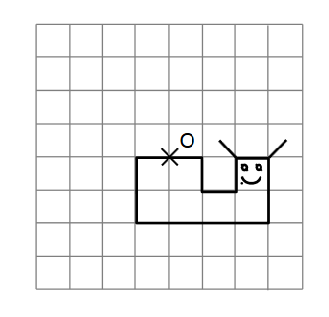
\includegraphics[scale=1]{symcentrale2.eps} 
\end{flushright}

\emul


\vspace*{0.5cm}

\exo{3,5}

\initq 
\q Construire un triangle ABC rectangle en A tel que  : AB = 5 cm et AC = 3 cm.\\

\q Tracer en vert le symétrique du triangle ABC par rapport au point B.\\

\q Tracer en bleu le symétrique du triangle ABC par rapport au point M, milieu de [AB].\\

\newpage

\vspace*{0.5cm}

\exo{1,5} (\textbf{sur le sujet}) Trouve le centre de symétrie lorsqu'il existe des figures ci-dessous. Trace le en \underline {bleu}.\\


\includegraphics[scale=0.9]{centresym.eps} \includegraphics[scale=1.2]{centresym2.eps} 
\includegraphics[scale=1.1]{centresym3.eps} 

\vspace*{0.5cm}

\exo{2}
DEF est un triangle isocèle en D tel que $\widehat{EDF} = 42,6$\degre. \\

Calculer la mesure des angles $\widehat{DEF}$ et $\widehat{DFE}$. \\

\vspace*{0.5cm}

\exo{3}\\
Le quadrilatère ABCD est un rectangle. Le point E appartient au segment [AB]. 

\begin{center}
\includegraphics[scale=0.7]{figangles.eps} 
\end{center}

Le triangle CDE est-il rectangle en E ? \textbf{Justifier votre réponse en trouvant les mesures de tous les angles du triangle CDE.} 

\end{document}
